\section{Scientific performance} \label{sec:sci-performance}

\subsection{Scientific production}

\subsubsection{Selected list of publications}

\autocite{Lamurias2015} \fullcite{Lamurias2015}
\begin{itemize}
    \item \textbf{Impact Factor}: 4.550
    \item \textbf{Non-self citations}: 19
\end{itemize}

\autocite{Pesquita2014} \fullcite{Pesquita2014}
\begin{itemize}
    \item \textbf{Impact Factor}: 2.262
    \item \textbf{Non-self citations}: 15
\end{itemize}

\autocite{Ferreira2013} \fullcite{Ferreira2013}
\begin{itemize}
    \item \textbf{Impact Factor}: 4.981
    \item \textbf{Non-self citations}: 20
\end{itemize}

\autocite{Ferreira2012a} \fullcite{Ferreira2012a}
\begin{itemize}
    \item \textbf{Impact Factor}: 3.501
    \item \textbf{Non-self citations}: 10
\end{itemize}

\autocite{Ferreira2010} \fullcite{Ferreira2010}
\begin{itemize}
    \item \textbf{Impact Factor}: 4.620
    \item \textbf{Non-self citations}: 43
\end{itemize}


\subsubsection{Histograms of publications}

\begin{figure}[H]
    \centering
    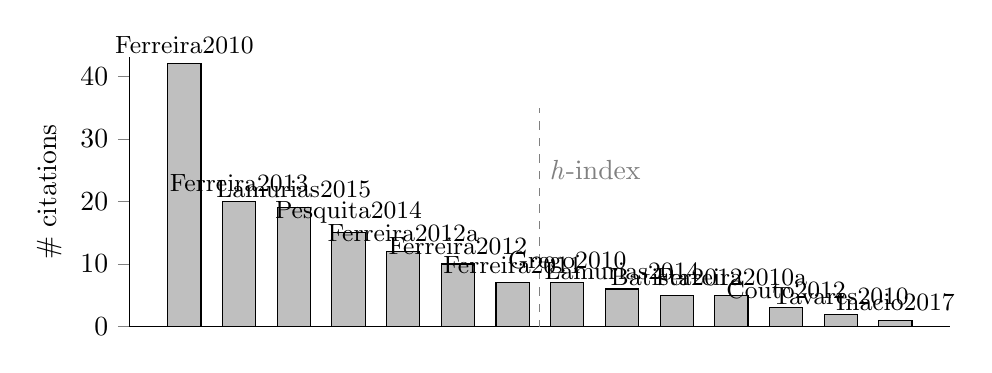
\begin{tikzpicture}
\begin{axis}[
    width=12cm,height=5cm,
    xmin=0,xmax=15,xminorticks=false,xmajorticks=false,
    ymin=0,ymax=43,
    ytick align=outside,
    axis x line*=bottom,axis y line*=left,
    tick label style={/pgf/number format/assume math mode=true},
    ylabel={\# citations},
    % enlargelimits=0.15,
    ybar,
    bar width=12pt,
]
\addplot[
    fill=lightgray,
    nodes near coords,
    point meta=explicit symbolic,
    every node near coord/.append style={font=\small}
]
    coordinates{
        (1,42) [\autocite{Ferreira2010}]
        (2,20) [\autocite{Ferreira2013}]
        (3,19) [\autocite{Lamurias2015}]
        (4,15) [\autocite{Pesquita2014}]
        (5,12) [\autocite{Ferreira2012a}]
        (6,10) [\autocite{Ferreira2012}]
        (7,7)  [\autocite{Ferreira2011}]
        (8,7)  [\autocite{Grego2010}]
        (9,6)  [\autocite{Lamurias2014}]
        (10,5) [\autocite{Batista2012}]
        (11,5) [\autocite{Ferreira2010a}]
        (12,3) [\autocite{Couto2012}]
        (13,2) [\autocite{Tavares2010}]
        (14,1) [\autocite{Inacio2017}]
    };
\addplot[gray,line legend,dashed,sharp plot,update limits=false]
    coordinates {
        (7.5,-3)
        (7.5,35)
    }
    node[right] at (7.5,25) {\textit{h}-index};

\end{axis}
\end{tikzpicture}

    \caption{Histogram of citations for each of my cited papers, with papers sorted from most cited to least cited. Top labels specify the publication according to Section~\ref{sec:publications}. The vertical dashed line shows the associated \textit{h}-index.}
    \label{fig:histogram-h-index}
\end{figure}

\begin{figure}[H]
    \centering
    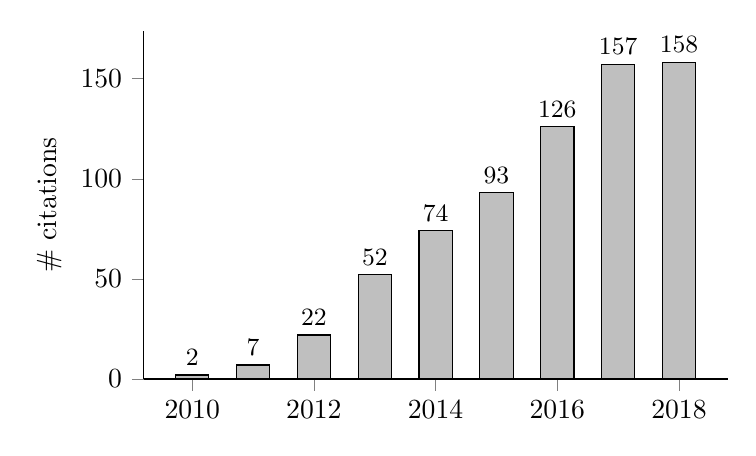
\begin{tikzpicture}
\begin{axis}[
    width=9cm,height=6cm,
    ymin=0,
    ytick align=outside,
    axis x line*=bottom,axis y line*=left,
    tick label style={
        /pgf/number format/assume math mode=true,
        /pgf/number format/1000 sep={}
    },
    ylabel={\# citations},
    % enlargelimits=0.15,
    ybar,
    bar width=12pt,
]
\addplot[
    fill=lightgray,
    nodes near coords,
    every node near coord/.append style={
        /pgf/number format/assume math mode=true,
        font=\small
    }
]
    coordinates{
        (2010,2)
        (2011,7)
        (2012,22)
        (2013,52)
        (2014,74)
        (2015,93)
        (2016,126)
        (2017,157)
        (2018,158)
    };

\end{axis}
\end{tikzpicture}

    \caption{Histogram showing the cumulative number of citations gathered throughout the years.}
    \label{fig:histogram-citations}
\end{figure}


\subsubsection{Selected list of citations}

\begin{refsection}[content/other.bib]
\fullciteorig{schulz2013concept}
\end{refsection}
\begin{itemize}
    \item Mentions my paper \autocite{Ferreira2012a} as \textbf{one of the twenty most influential papers} in the knowledge-representation, biomedical ontologies and electronic health issues, as listed by the members of the LinkedIn Working Group on Medical Concept Representation.
\end{itemize}

\begin{refsection}[content/other.bib]
\fullciteorig{hastings2013chebi}
\end{refsection}
\begin{itemize}
    \item This paper is a major milestone in Chemoinformatics, describing ChEBI (an ontology of chemical compounds). It has itself 163 citations. Cites my paper \autocite{Ferreira2010} as an example of an \textbf{application that makes use of the semantic information} encoded in ChEBI for automatic classification.
\end{itemize}

\begin{refsection}[content/other.bib]
\fullciteorig{hastings2012structure}
\end{refsection}
\begin{itemize}
    \item This paper expresses \textbf{the need and usefulness of systems that exploit the machine-readable information} provided by reference ontologies, and cites my paper \autocite{Ferreira2010} as an example.
\end{itemize}

\begin{refsection}[content/other.bib]
\fullciteorig{wegner2012cheminformatics}
\end{refsection}
\nobreakhere
\begin{itemize}
    \vspace{\topsep}
    \item This paper advocates the use of \textbf{open-source solutions to deal with the vast amount of existing chemical information}, mentioning semantic similarity in ChEBI and citing my paper \autocite{Ferreira2010}.
\end{itemize}

\begin{refsection}[content/other.bib]
\fullciteorig{hoehndorf2014thematic}
\end{refsection}
\begin{itemize}
    \item This paper aims ``to disseminate the latest developments in research on biomedical ontologies and provide a venue for publishing newly developed ontologies, updates to existing ontologies as well as methodological advances, and selected contributions from conferences and workshops''. It cites my paper \autocite{Ferreira2010} as an example of a semantic similarity application and my paper \autocite{Ferreira2013} as \textbf{the start of using more than taxonomies in semantic similarity} in the biomedical domain.
\end{itemize}


% \subsubsection{Citation metrics}
% \vspace{-1.5\baselineskip}
% \begin{table}[H]
%     \centering
%     \caption{Citation metrics computed using Google Scholar and DBLP data.}
%     \label{tab:citation-metrics}
%     \begin{tabular}{llr}
%     \toprule
%      & \textbf{Metric} & \textbf{Value} \\
%     \midrule
%     Google Scholar & \textit{h}-index & 6 \\
%                    & i10-index        & 2 \\
%                    & citations        & 92 \\
%                    & cited papers     & 14 \\
%     \addlinespace
%     DBLP & co-authors           & 15 \\
%          & \#journal articles   & 5 \\
%          & \# conference papers & 6 \\
%     \bottomrule
%     \end{tabular}
% \end{table}


\subsubsection{Open Software}

\entry
  [2015]
  [URL: \url{http://github.com/jdferreira/owltosql}]
  {OWLtoSQL}
\begin{itemize}
    \item This software is one of the results of my PhD work. It is used to \textbf{convert an ontology written in OWL} (Web Ontology Language) \textbf{into a relational database}, which offers several advantages, the most prominent of which is that it enables \emph{random} access to the ontology constituents (classes, properties, axioms, \emph{etc.}). It has been used by Bruno Inácio in his M.Sc work (see Section~\ref{sub:academic-supervision}).
\end{itemize}


\entry
    [2015]
    [URL: \url{http://github.com/jdferreira/mossy.bak}]
    {Multi-domain Ontology-based Semantic Similarity (MOSSy)}
\begin{itemize}
    \item This software also resulted from my PhD work. It is responsible for calculating \textbf{semantic similarity between resources annotated with concepts from multiple ontologies}. The program is configurable to use any OWL ontology and can handle any type of annotated resource, both in single- and multi-domain contexts. It is extensible, since it allows the implementation of semantic similarity measures as Python classes.
\end{itemize}


\subsubsection{Knowledge representation artefacts}

\entry
    [2013]
    [See my paper \autocite{Ferreira2012a}]
    {Network of Epidemiology-Related Ontologies}
\begin{itemize}
    \item This work is a \textbf{collection of ontologies related to the epidemiology domain}. It contains 13 ontologies, from domains such as biochemistry, diseases, environment, transmission, vaccines, and geography, which provide the necessary concepts to annotate a digital resource of the epidemiological domain. The network was later included in the Epimarketplace, a repository of epidemic resources, in order to facilitate the annotation process.
    \item \textbf{Developed}: during my work in the EPIWORK project.
\end{itemize}

\entry
    [2014]
    [URL: \url{https://code.google.com/p/epidemiology-ontology/}]
    {Epidemiology Ontology}
\begin{itemize}
    \item This ontology represents both \textbf{disease transmission methods and epidemiology parameters}, containing over 300 concepts. This ontology fills the previously existing gap~in these areas, which were under-represented in biomedical ontologies. It supports the semantic annotation of resources.
    \item \textbf{Developed}: during my work in the EPIWORK project.
\end{itemize}


\subsection{Research projects}

\subsubsection{Past projects} \label{ss:past-projects}

\entry
    [2016-2019]
    [URL: \url{http://lasige.di.fc.ul.pt/Projects/SMiLax}]
    {Semantic Mining with Linked Data (SMiLax)}
\begin{itemize}
    \item \textbf{Position}: Member of research team
    \item \textbf{Funding}: FCT (82$\;$714€)
    \item \textbf{Grant}: PTDC/EEI-ESS/4633/2014
    \item \textbf{Description of project}: This project will improve the state of the art in semantic data mining by establishing novel methods and algorithms for the automated semantic annotation and enrichment of data, whose output will be explored by novel data mining approaches capable of capitalizing on the semantic web.
    \item \textbf{My contributions}: I am involved in research to improve current ontology-matching algorithms using semantic similarity instead of background knowledge.
\end{itemize}

\entry
    [2012-2014]
    [URL: \url{http://somer.rd.ciencias.ulisboa.pt/}]
    {Semantic Ontology Matching using External Resources (SOMER)}
\begin{itemize}
    \item \textbf{Position}: Member of research team
    \item \textbf{Funding}: FCT (84$\;$000€)
    \item \textbf{Grant}: PTDC/EIA-EIA/119119/2010
    \item \textbf{Description of project}: The SOMER project aimed to develop ontology matching methods that exploit external knowledge resources through evidence and information content provided by unstructured text and annotation corpora. The results were applied to real world applications based on existing ontologies in the biomedical and geospatial areas.
    \item \textbf{My contributions}: I was involved in writing the proposal for this project. I was also responsible for exploring ways that allowed the use of semantic similarity measures in the process of ontology matching. I contributed to 1 peer-reviewed publication.
\end{itemize}

\entry
    [2009-2013]
    [URL: \url{http://xldb.di.fc.ul.pt/wiki/EPIWork}]
    {Developing the Framework for an Epidemic Forecast Infrastructure (EPIWORK)}
\begin{itemize}
    \item \textbf{Position}: Hired researcher
    \item \textbf{Funding}: FP7 (5$\;$000$\;$000€)
    \item \textbf{Grant}: 231807
    \item \textbf{Description of project}: The EPIWORK project proposed a framework of tools and knowledge for the design of epidemic forecast infrastructures, including: development of the mathematical and computational methods needed to achieve prediction of disease spreading in complex social systems; development of large scale, data driven computational models aimed at epidemic scenario forecast; design and implementation of data-collection mechanisms, such as the collection of real-time disease incidence, through innovative web and ICT applications; and the implementation of a computational platform for epidemic research and data sharing.
    \item \textbf{My contributions}: The LASIGE team was responsible for the creation go the Epidemic Marketplace, an online platform for epidemic research and data sharing was the data-hub for the multiple research communities and countries involved in the project. I was hired by the LASIGE team as a consultant in semantic web, specifically to design the semantic metadata model that was used to annotate the resources of the marketplace, as well as to design the Network of Epidemiology-Related Ontologies, which contributed to the repository as a collection of concepts used to annotate the resources. I contributed to 5 peer-reviewed publications and 1 open-source ontology.
\end{itemize}

\entry
    [2010]
    {Geographic Reasoning for Search Engines II (GREASE-II)}
\begin{itemize}
    \item \textbf{Position}: M.Sc fellowship
    \item \textbf{Funding}: FCT (117$\;$300 €)
    \item \textbf{Grant}: PTDC/EIA/73614/2006
    \item \textbf{Description of project}: This project aimed at researching information access methods to large collections of documents and objects having geographically rich text and meta-data. One of the main ideas of the project was that geospatial information can be mapped into ontology concepts.
    \item \textbf{My contributions}: One of the tasks of this project was to perform text-mining directly onto news reports in order to find geographical references in text; to assist in this task, a disambiguation module had to be created. I was assigned the creation of software to help disambiguate annotations manually, which would then later be used in a machine-learning step. I was also tasked with the alignment of Geo-Net-PT (a geographical ontology of the Portuguese territory) to Yahoo! GeoPlanet™ (an infrastructure for geo-referencing data on the Internet). I contributed to 1 technical report and to 1 open-source software.
\end{itemize}


\subsubsection{International Collaborations}

\entry[2016-2017]{European Bioinformatics Institute (EBI)}
\begin{itemize}
    \item I collaborated with the team behind MetaboLights, a repository used to store details of experiments related to research in metabolism and information derived from the research. My role in this collaboration was to help \textbf{devise ways to measure annotation quality} in order find resources under-annotated and to help authors submit properly annotated data. This collaboration resulted in 1 conference publication~\autocite{Inacio2017} and 1 peer-reviewed publication~\autocite{Ferreira2017}.
\end{itemize}

\entry[2013-2015]{University College London (UCL)}
\begin{itemize}
    \item I collaborated with Bernard D. Bono, a Principal Research Fellow in Health Informatics in UCL, in several fronts. The most recent collaboration is related to the \textbf{digital representation of functional tissue units} (small portions of an organ that perform a certain biological function) and the ways to compare them and publish them in a knowledge-base. This collaboration resulted in an oral presentation at the Virtual Physiological Human Conference 2014~\autocite{Ferreira2014}.
\end{itemize}

\entry[2013]{European Bioinformatics Institute (EBI)}
\begin{itemize}
    \item I collaborated with J. Hastings, former group coordinator of the Chemoinformatics and Metabolism Team at EBI, in devising a semantic similarity measure that can effectively \textbf{capture the information provided by the disjointness axioms of an ontology}. This collaboration resulted in 1 peer-reviewed publication~\autocite{Ferreira2013}.
\end{itemize}

\entry[2012]{Institute for Scientific Interchange (ISI) Foundation}
\begin{itemize}
    \item I collaborated with Daniela Paolotti, the Project manager of the Italian web platform for Influenza-like Illness Surveillance. This collaboration resulted from my position at EPIWORK, and resulted in the publication of 1 peer-reviewed publication detailing \textbf{how to introduce semantic web technologies and ideas in the epidemiology domain}~\autocite{Ferreira2012a}.
\end{itemize}


\subsection{Academic supervision} \label{sub:academic-supervision}

\subsubsection{Current supervision}

\entry
    [2017-2020]
    [University of Lisbon]
    {PhD in Statistics}
\begin{itemize}
    \item \textbf{Student}: Joana Estevens
    \item \textbf{Position}: Co-supervisor with Dr. Teresa Alpuim, University of Lisbon
    \item \textbf{Thesis}: ``Application of machine-learning in vehicle insurance'' (loosely translated from the official Portuguese title: ``Aplicação de métodos de aprendizagem automática no desenvolvimento de um novo produto de seguro automóvel'')
    \item \textbf{Topic}: The work proposes the application of generalized linear models and machine learning algorithms in data from an insurance company regarding vehicle insurance. The final aim of this work is the establishment of customized insurance rates for every client, where the actual premium is calculated based on the values of a large number of variables not usually used in this area, thus creating an insurance policy that is more tailored to the client's accident probability and more just to all clients in general.
\end{itemize}


\subsubsection{Past supervision}

\entry
    [2016-2017]
    [University of Lisbon]
    {M.Sc in Informatics Engineering}
\begin{itemize}
    \item \textbf{Student}: Isabela Mott
    \item \textbf{Position}: Co-supervisor with Dr Catia Pesquita, University of Lisbon
    \item \textbf{Thesis}: ``AML-SSM: Semantic Similarity for Ontology Alignment''
    \item \textbf{Topic}: As part of my participation in the SMiLax project (see section~\ref{ss:past-projects}), I supervised the extension of the existing AgreementMaker Light (AML) platform, one of the most performant Ontology Alignment (OA) software pieces for biomedical ontologies. The student  repurposed the idea of semantic similarity in order to further improve the existing OA algorithms in AML.
\end{itemize}


\entry
    [2015-2016]
    [University of Lisbon]
    {M.Sc in Informatics Engineering}
\begin{itemize}
    \item \textbf{Student}: Bruno Inácio
    \item \textbf{Position}: Co-supervisor with Dr Francisco M. Couto, University of Lisbon
    \item \textbf{Thesis}: ``How much is metadata worth?'' (loosely translated from the official Portuguese title: ``Quanto valem os metadados?'')
    \item \textbf{Topic}: The work focused (i)~on the study of the quality of metadata as a way to sustain semantic integration and to facilitate data-sharing, based on the specificity of the ontology concepts used to annotate the resources and on the thoroughness of these annotations; and (ii)~on the development of a platform that allows the assessment of metadata quality of the resources in a scientific data repository.
\end{itemize}


\entry
    [2011-2012]
    [University of Lisbon]
    {Internship of a B.Sc in Biochemistry}
\begin{itemize}
    \item \textbf{Student}: Hugo Ferreira
    \item \textbf{Position}: Co-supervisor with Dr Francisco M. Couto, University of Lisbon
    \item \textbf{Topic}: Creation of an ontology of epidemiology.
    \item \textbf{Topic}: The work consisted in using the textual descriptions in a Dictionary of Epidemiology to find relationships between the concepts and thus create an ontology of epidemiology.
\end{itemize}


\subsection{Scientific Dissemination}

\subsubsection{Conference organisation}

\entry
    [2015]
    [Workshop \& tutorial chair, Proceedings chair]
    {6\textsuperscript{th} International Conference on Biomedical Ontology (ICBO)}
\begin{itemize}
    \item \textbf{Description}: The sixth International Conference on Biomedical Ontology (ICBO) was held in Lisbon in 2015 (\url{http://icbo2015.fc.ul.pt}). This prestigious and well-attended conference gathered multidisciplinary researchers at the University de Lisbon to present and discuss the latest research breakthroughs in exploring ontologies in a biomedical and clinical context.
    \item \textbf{Position}: Part of the organization; I was Workshop \& tutorial chair and Session chair. I was also part of the Proceedings team, having compiled the Proceedings, and organized the submission to CEUR-WS.
\end{itemize}
\vspace{-5mm}

\subsubsection{Reviewer}

\begin{yeartable}
    2018 & Oxford Bioinformatics \\
    2017 & Journal of Biomedical Semantics \\
         & Journal of Epidemiology \& Community Health \\
    2016 & Journal of Biomedical Semantics \\
    2015 & Journal of Biomedical Semantics \\
         & Journal of Epidemiology \& Community Health \\
    2013 & Oxford Bioinformatics \\
    2012 & Oxford Bioinformatics \\
\end{yeartable}


\subsubsection{Program Committee and other reviewer activities}

\begin{yeartable}
    2018 & Conference on Practical Applications of Computational Biology \& Bioinformatics \\
    2017 & Conference on Practical Applications of Computational Biology \& Bioinformatics \\
    2015 & Bioinformatics Open Days \\
         & Conference on Practical Applications of Computational Biology \& Bioinformatics \\
         & Portuguese Conference on Artificial Intelligence \\
    2014 & Conference on Practical Applications of Computational Biology \& Bioinformatics \\
         & International Conference on Data Integration \& Life Sciences \\
\end{yeartable}


\subsection{Grants, Honors and Awards}

\subsubsection{Grants}

\begin{yeartable}
    2010--2015 & PhD Grant by Fundação para a Ciência e Tecnologia (the Portuguese Science Funding Agency)  \\
    2009--2010 & Pre-PhD grant by LASIGE \\
\end{yeartable}


\subsubsection{Awards}

\begin{yeartable}
    2014 & BPH Travel Award by the VPH Institute \\
    2006 & Best Student in 1\textsuperscript{st} year by University of Lisbon \\
\end{yeartable}


